\documentclass[11pt,a4paper]{article}

\usepackage[T1]{fontenc}
\usepackage{lmodern}
\usepackage[margin=2.5cm]{geometry}
\usepackage{graphicx}
\usepackage{booktabs}
\usepackage{tabularx}
\usepackage{array}
\usepackage{float}
\usepackage{needspace}
\usepackage[font=small,labelfont=bf]{caption}
\usepackage{fancyhdr}
\usepackage{amsmath}
\usepackage{xcolor}
\usepackage[colorlinks=true,linkcolor=black,urlcolor=blue]{hyperref}

\graphicspath{{figs/}}
\setlength{\parindent}{0pt}
\setlength{\parskip}{6pt}

\pagestyle{fancy}
\fancyhf{}
\lhead{COL334 Assignment 4}
\rhead{2024CS10300 \,\&\, 2024CS10582}
\cfoot{\thepage}
\renewcommand{\headrulewidth}{0.4pt}

\newcommand{\cmd}[1]{\texttt{#1}}
\newcommand{\question}[2]{\subsubsection*{Q#1.\ #2}}
\newcommand{\shot}[3][0.85]{%
  \begin{figure}[H]\centering
  \includegraphics[width=#1\linewidth]{#2}
  \caption{#3}
  \end{figure}}

\begin{document}

\begin{titlepage}
\centering
\vspace*{3cm}
{\large Department of Computer Science and Engineering, IIT Delhi\par}
\vspace{1cm}
{\Large\bfseries COL334 Assignment 4\par}
\vspace{0.4cm}
{\LARGE Make the Network Find its Way\par}
\vspace{0.4cm}
{\large Static Routing, RIPv2 and OSPF in Cisco Packet Tracer\par}
\vspace{2cm}
\begin{tabular}{ll}
\toprule
\textbf{Name} & \textbf{Entry number} \\
\midrule
Yashwardhan Singh Choudhary & 2024CS10300 \\
Tejasvi Shrivastava & 2024CS10582 \\
\bottomrule
\end{tabular}
\vfill
Packet Tracer version: 9.0.1.0858
\end{titlepage}

\section*{Setup}

The network (four Cisco 2911 routers R1--R4, four PCs, five router-to-router links and four
LANs) was built exactly as in Tables~1 and~2 of the assignment and saved as
\cmd{base.pkt}. R2 is the DCE end of the R2--R3 serial link (clock rate 128000),
Serial0/0/1 on R2 and R3 is shut down, and every router carries the banner
\cmd{2024CS10300 2024CS10582}. Before saving, every router pinged the far end of each of
its links and every PC pinged its default gateway. Parts A, B and C each start from a fresh
copy of \cmd{base.pkt}. In all route-table screenshots the route to LAN~D
(192.168.4.0/24) is marked with a red box.

%=====================================================================
\section{Part A: Static Routing}

Each router has exactly three static routes in next-hop form, one to each remote LAN. The
next hop is the neighbour that owns the LAN, except R1$\to$LAN~D and R4$\to$LAN~A, which go
via R2.

\shot[0.6]{fig1}{Part A: PC-A pings PC-B (192.168.2.10), PC-C (192.168.3.10) and PC-D (192.168.4.10) successfully, followed by \cmd{tracert 192.168.4.10}.}
\shot{fig2}{Part A: R1 \cmd{show ip route}. The static route to LAN~D (boxed) is \cmd{S 192.168.4.0/24 [1/0] via 10.0.12.2}.}

\question{1}{Addresses printed by \cmd{tracert 192.168.4.10} on PC-A}
192.168.1.1 $\to$ 10.0.12.2 $\to$ 10.0.24.2 $\to$ 192.168.4.10 (R1, R2, R4, PC-D). The TTL of 125 in
the replies from PC-D ($128 - 3$ routers) confirms three router hops.

\question{2}{Next hop used by R1 for LAN D}
10.0.12.2 (R2), as required by rule S4.

%=====================================================================
\section{Part B: RIPv2}

All four routers run \cmd{router rip} with \cmd{version 2} and \cmd{no auto-summary}, and
advertise their networks with \cmd{network 10.0.0.0} and their own LAN. RIP network
statements are classful, so 10.0.0.0 covers all of a router's 10.0.x.x/30 links. No static
routes are configured.

\shot{fig3}{Part B: R1 \cmd{show ip route} after convergence. Routes marked R are learned through RIP (administrative distance 120). The route to LAN~D (boxed) has hop count 2 and two next hops.}

\question{3}{Hop count and next hops of R1's route to 192.168.4.0/24}
Hop count 2, next hops 10.0.12.2 (via R2) and 10.0.13.2 (via R3). Both paths, R1-R2-R4
and R1-R3-R4, are two hops long. RIP's metric ignores link speed, so the paths tie, and IOS
installs both and load-balances across them.

\question{4}{How R1 learns the route without a static route}
RIPv2 is a distance-vector protocol. Every router sends its routing table to its neighbours
every 30 seconds (RIPv2 uses multicast 224.0.0.9). R4 advertises its directly connected
network 192.168.4.0/24 to R2 and R3, which install it with hop count 1 and include it in
their own updates to R1. R1 adds one hop to each advertised metric, giving hop count 2
via both R2 (10.0.12.2) and R3 (10.0.13.2). Because the two metrics are equal, both are
installed. The route is marked R with administrative distance 120, and it is refreshed by
each periodic update, so no manual configuration of the route itself is needed.

%=====================================================================
\section{Part C: OSPF and Link Costs}

All routers run OSPF process 1 in area 0, with one \cmd{network} statement per directly
connected network (e.g.\ \cmd{network 10.0.12.0 0.0.0.3 area 0},
\cmd{network 192.168.1.0 0.0.0.255 area 0}). The costs of Table~3 are set with
\cmd{ip ospf cost} on both ends of every router-to-router link, and LAN interfaces keep
their default cost of 1.

\textit{Note on cost 1:} on a GigabitEthernet interface the default OSPF cost in Packet
Tracer is already 1 (100~Mbps reference $\div$ 1000~Mbps, rounded up). Because
\cmd{ip ospf cost 1} equals the default, Packet Tracer does not show it in
\cmd{show running-config}, even though it was entered. The serial cost of 1 is shown
because the serial default is different. Figure~\ref{fig:cost} confirms that the cost is
applied.

\subsection{Plan A}

\shot{fig4}{Plan A: R1 \cmd{show ip route}. Route to LAN~D (boxed): \cmd{O 192.168.4.0/24 [110/3] via 10.0.12.2}.}
\shot{fig5}{Plan A: \cmd{tracert 192.168.4.10} from PC-A follows R1 (192.168.1.1), R2 (10.0.12.2), R4 (10.0.24.2), PC-D.}
\begin{figure}[H]\centering
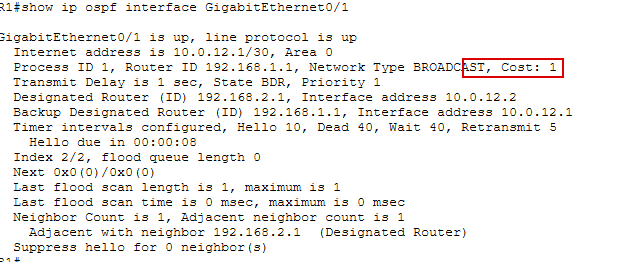
\includegraphics[width=0.75\linewidth]{fig6}
\caption{Plan A: \cmd{show ip ospf interface GigabitEthernet0/1} on R1 reports \cmd{Cost: 1} (boxed), confirming the configured R1--R2 cost.}
\label{fig:cost}
\end{figure}

\question{5}{Path and metric under Plan A}
Path R1-R2-R4, metric 3.

\question{6}{How the metric is obtained}
OSPF adds the cost of each outgoing interface on the way to the destination network: R1
G0/1 (R1$\to$R2) = 1, plus R2 G0/2 (R2$\to$R4) = 1, plus R4 G0/0 (LAN~D, default) = 1, which
gives 3.

\question{7}{Why this path is preferred over R1-R3-R4}
R1-R3-R4 costs R1 G0/2 (5) + R3 G0/2 (5) + R4 G0/0 (1) = 11. OSPF runs Dijkstra's
shortest-path-first algorithm over its link-state database and installs only the lowest-cost
path. Since $3 < 11$, R1-R2-R4 is chosen, even though both paths have the same number of
hops. For the same reason, only one next hop (10.0.12.2) appears, unlike the two equal
next hops RIP showed.

\subsection{Plan B}

\shot{fig7}{Plan B: R1 \cmd{show ip route}. Route to LAN~D (boxed): \cmd{O 192.168.4.0/24 [110/11] via 10.0.13.2}.}
\shot[0.75]{fig8}{Plan B: \cmd{tracert 192.168.4.10} from PC-A follows R1, R3 (10.0.13.2), R4 (10.0.34.2), PC-D.}

\question{8}{Path and metric under Plan B, and why}
Path R1-R3-R4, metric 11. Raising the R1--R2 and R2--R4 costs to 10 makes every path
that uses them more expensive. The candidate paths (outgoing interface costs, including
LAN~D's cost of 1) are:

\begin{table}[H]\centering
\begin{tabular}{ll}
\toprule
\textbf{Path} & \textbf{Cost} \\
\midrule
R1-R2-R4    & $10 + 10 + 1 = 21$ \\
R1-R2-R3-R4 & $10 + 1 + 5 + 1 = 17$ \\
R1-R3-R2-R4 & $5 + 1 + 10 + 1 = 17$ \\
R1-R3-R4    & $5 + 5 + 1 = \mathbf{11}$ \\
\bottomrule
\end{tabular}
\end{table}

SPF picks the lowest-cost path, R1-R3-R4. The topology and hop counts did not change,
only the costs, and that alone moved the traffic. The same effect is visible for LAN~B, which
R1 now reaches through R3 and the serial link at cost 7 instead of through its direct R1--R2
link at cost 11.

%=====================================================================
\section{Part D: Link Failure (R2 GigabitEthernet0/2 shut down)}

\subsection{OSPF (starting from Plan A)}

\needspace{10\baselineskip}
\textbf{Before the failure} (Plan A, from Part C):

\shot{fig9}{OSPF before failure: R1 \cmd{show ip route}, LAN~D at [110/3] via 10.0.12.2 (boxed).}
\shot[0.75]{fig10}{OSPF before failure: \cmd{ping 192.168.4.10} from PC-A succeeds (TTL 125, three routers).}

\needspace{10\baselineskip}
\textbf{After the failure} (saved as \cmd{partD\_ospf\_linkdown.pkt}):

\shot{fig11}{OSPF with R2--R4 down: R1 \cmd{show ip route}. 10.0.24.0/30 has disappeared and LAN~D is now [110/8] via 10.0.12.2 (boxed).}
\shot[0.65]{fig12}{OSPF with R2--R4 down: \cmd{ping 192.168.4.10} from PC-A succeeds (TTL 124, four routers).}
\shot[0.7]{fig13}{OSPF with R2--R4 down: \cmd{tracert} shows the detour R1, R2 (10.0.12.2), R3 over the serial link (10.0.23.2), R4 (10.0.34.2), PC-D.}

\needspace{10\baselineskip}
\textbf{After the link is restored} (\cmd{no shutdown}, state not saved):

\shot[0.7]{fig14}{OSPF after restoring the link: LAN~D back at [110/3] via 10.0.12.2 (boxed), and 10.0.24.0/30 is back.}
\shot[0.7]{fig15}{OSPF after restoring the link: \cmd{ping 192.168.4.10} from PC-A succeeds again with TTL 125.}

\question{9}{OSPF with the link down}
Yes, PC-A can still reach PC-D. R1 uses R1-R2-R3-R4 with metric 8 = R1 G0/1 (1) + R2
S0/0/0 (1) + R3 G0/2 (5) + R4 G0/0 (1). The other surviving path, R1-R3-R4, costs
$5 + 5 + 1 = 11$, so OSPF still goes through R2 and then the cheap serial link to R3. The next
hop stays 10.0.12.2, so the change is visible only in the metric ($3 \to 8$) and in the
\cmd{tracert}.

\question{10}{How R1's OSPF table changes after the failure and after restoration}
\textit{After the failure:} R2 and R4 detected the interface going down and flooded updated
router LSAs, and every router reran SPF within seconds. In R1's table, 10.0.24.0/30
disappeared (7 subnets became 6), and the LAN~D route changed from [110/3] to [110/8].
The next hop stayed 10.0.12.2, but traffic now continues R2 $\to$ R3 $\to$ R4. Routes that never
used the R2--R4 link (LAN~B, LAN~C, 10.0.23.0/30) were unchanged. 10.0.34.0/30 kept
metric 7 but is now reached through R2 and the serial link to R3 instead of through R4.

\textit{After restoration:} the R2--R4 adjacency re-formed, new LSAs were flooded, and SPF
restored the original routes: LAN~D at [110/3] via R1-R2-R4, and 10.0.24.0/30 at [110/2].
These two routes have younger ages (00:05:36) than the rest of the table, which shows
they were just relearned. Both changes took effect almost immediately, with no hold-down
period.

\subsection{RIPv2 (starting from Part B)}

\needspace{10\baselineskip}
\textbf{Before the failure} (from Part B):

\shot{fig16}{RIPv2 before failure: R1 \cmd{show ip route}, LAN~D at [120/2] via 10.0.12.2 and 10.0.13.2 (boxed).}
\shot[0.6]{fig17}{RIPv2 before failure: PC-A pings PC-B, PC-C and PC-D (192.168.4.10) successfully.}

\needspace{10\baselineskip}
\textbf{After the failure}, recorded after advancing more than 4 minutes of simulated time
(saved as \cmd{partD\_rip\_linkdown.pkt}):

\shot[0.7]{fig18}{RIPv2 with R2--R4 down: R1 \cmd{show ip route}. LAN~D is [120/2] via 10.0.13.2 only (boxed), and 10.0.24.0/30 is gone.}
\shot[0.65]{fig19}{RIPv2 with R2--R4 down: \cmd{ping 192.168.4.10} from PC-A succeeds (TTL 125).}
\shot[0.7]{fig20}{RIPv2 with R2--R4 down: \cmd{tracert} follows R1, R3 (10.0.13.2), R4 (10.0.34.2), PC-D.}

\question{11}{RIPv2 with the link down}
Yes, connectivity returns. R1's route to LAN~D has hop count 2 and a single next hop,
10.0.13.2 (path R1-R3-R4). Before the failure, R1 had two equal 2-hop routes, via R2 and
via R3. When the R2--R4 link failed, R2 lost its 1-hop route to LAN~D, and the only
alternative it still had was through R3, which would cost R1 3 hops. RIP keeps only the
routes with the fewest hops, so the R2 next hop was removed and the 2-hop path via R3
remains.

\question{12}{Comparison of RIPv2 and OSPF in this experiment}
Both protocols restored PC-A to PC-D connectivity without any manual route changes, but
they behaved differently.

\textit{Speed.} OSPF routers detected the failure, flooded LSAs and
reran SPF, so R1's table changed almost immediately, and the original path returned just
as quickly after restoration. RIPv2 learns of changes only through periodic updates (every
30\,s), and its invalid and hold-down timers (180\,s) delay new information. The assignment
therefore required advancing 4 minutes before recording results, and a RIP table can look
stable while still waiting to change.

\textit{Path chosen.} OSPF chose R1-R2-R3-R4 (cost 8) and
used the low-cost serial link even though that path has 3 hops. RIPv2 chose R1-R3-R4
because it is the only remaining 2-hop path. The same failure therefore produced different
paths, because the protocols measure ``best'' differently: total configured cost for OSPF,
number of hops for RIP.

%=====================================================================
\section{Part E: Comparison (Table 4)}

\begin{table}[H]\centering\small
\renewcommand{\arraystretch}{1.3}
\begin{tabularx}{\linewidth}{>{\raggedright\bfseries}p{2.4cm}
  >{\raggedright\arraybackslash}X >{\raggedright\arraybackslash}X >{\raggedright\arraybackslash}X}
\toprule
Property & \textbf{Static routing} & \textbf{RIPv2} & \textbf{OSPF} \\
\midrule
How are routes obtained? &
Typed manually by the administrator with \cmd{ip route} on each router (3 per router, 12 in total in Part A). &
Learned from neighbours: each router periodically (every 30\,s) sends its routing table (distance vector), and the receiver adds 1 hop. &
Each router floods LSAs describing its links, builds an identical link-state database, and computes routes with Dijkstra's SPF algorithm. \\
\midrule
Adapts automatically to a failed link? &
No. Routes stay until the administrator changes them, so with the static routes from Part A, traffic over a failed R2--R4 link would be dropped. &
Yes, but slowly. Changes spread through periodic updates and are delayed by invalid/hold-down timers (180\,s). In Part D, results were only reliable after waiting 4 minutes. &
Yes, quickly. The failure is flooded as LSAs and SPF reruns within seconds (Part D), and the original path returns as fast once the link is restored. \\
\midrule
What determines the preferred path? &
The administrator's choice of next hop in each route. &
Lowest hop count (max 15). Link speed is ignored, and equal-hop paths are load-balanced (two next hops in Part B). &
Lowest total cost, the sum of outgoing interface costs (\cmd{ip ospf cost} or reference bandwidth $\div$ bandwidth). Changing the costs alone moved the path in Plan B. \\
\midrule
What must an administrator configure? &
Every route to every remote network on every router, and updates whenever the topology changes. &
\cmd{router rip}, \cmd{version 2}, \cmd{no auto-summary}, and classful \cmd{network} statements on each router. &
\cmd{router ospf <process>}, \cmd{network <address> <wildcard> area <n>} for each network, and optionally \cmd{ip ospf cost} to steer traffic. \\
\bottomrule
\end{tabularx}
\end{table}

%=====================================================================
\section{Part F: Reflection}

\question{13}{Two slow links versus three fast links}
RIP \emph{would} prefer the route with two slow links, because its only metric is hop count: 2
hops beats 3, whatever the link speeds. OSPF \emph{might} prefer the three fast links,
because it chooses the lowest total cost, and by default an interface's cost is reference
bandwidth $\div$ interface bandwidth. For example, with the default 100~Mbps reference, two
10~Mbps links cost $10 + 10 = 20$, while three 100~Mbps links cost $1 + 1 + 1 = 3$, so OSPF
picks the three-link path. It is only ``might'' because the result depends on the costs: an
administrator can set \cmd{ip ospf cost} manually, and links faster than the reference bandwidth
all get cost 1 unless the reference is raised. Plan B showed this: changing only the costs
moved R1's path from R1-R2-R4 to R1-R3-R4, which RIP could never do.

\question{14}{Manually configuring routes in a network with hundreds of routers}
Every router needs a route to every network it is not directly connected to, so the number
of static routes grows roughly as routers $\times$ networks, which means thousands of entries to
type and maintain. Human error becomes likely: a wrong next hop or a missing route
causes black holes or routing loops that are hard to trace. Static routes do not react to
failures. When a link goes down, traffic is dropped until an administrator edits routes on
many routers, unlike in Part D where RIP and OSPF recovered on their own. Adding a
network or changing the topology means updating many routers consistently and in the
right order. Paths are also harder to optimise and keep symmetric, and the configuration is
hard to audit. Dynamic routing protocols exist to automate exactly this.

\end{document}
